\begin{frame}
  \frametitle{I Need Super Computer Time For My Featureless App}
  \begin{itemize}
    \item JavaScript is more \textit{unsafe} than Rust, due of a lack of typing
      and restrictions
  \end{itemize}
\end{frame}

\begin{frame}
  \frametitle{I Need Super Computer Time For My Featureless App}
  \begin{itemize}
    \item JavaScript is more \textit{unsafe} than Rust, due of a lack of typing
      and restrictions
    \item Need to decode the output from the modules, and catch any exceptions
  \end{itemize}
\end{frame}

\begin{frame}
  \frametitle{I Need Super Computer Time For My Featureless App}
  \begin{itemize}
    \item JavaScript is more \textit{unsafe} than Rust, due of a lack of typing
    \item Need to decode the output from the modules, and catch any exceptions
    \item When implementing the init \to update \to view - cycle, I tested with
      a \textit{basic} module, which should only display "Hello, World!"
  \end{itemize}
\end{frame}

\begin{frame}
  \frametitle{I Need Super Computer Time For My Featureless App}
  \begin{itemize}
    \item JavaScript is more \textit{unsafe} than Rust, due of a lack of typing
    \item Need to decode the output from the modules, and catch any exceptions
    \item When implementing the init \to update \to view - cycle, I tested with
      a \textit{basic} module, which should only display "Hello, World!"
      \begin{itemize}
        \item The module initialized the state
      \end{itemize}
  \end{itemize}
\end{frame}

\begin{frame}
  \frametitle{I Need Super Computer Time For My Featureless App}
  \begin{itemize}
    \item JavaScript is more \textit{unsafe} than Rust, due of a lack of typing
    \item Need to decode the output from the modules, and catch any exceptions
    \item When implementing the init \to update \to view - cycle, I tested with
      a \textit{basic} module, which should only display "Hello, World!"
      \begin{itemize}
        \item The module initialized the state
        \item It rendered the view
      \end{itemize}
  \end{itemize}
\end{frame}

\begin{frame}
  \frametitle{I Need Super Computer Time For My Featureless App}
  \begin{itemize}
    \item JavaScript is more \textit{unsafe} than Rust, due of a lack of typing
    \item Need to decode the output from the modules, and catch any exceptions
    \item When implementing the init \to update \to view - cycle, I tested with
      a \textit{basic} module, which should only display "Hello, World!"
      \begin{itemize}
        \item The module initialized the state
        \item It rendered the view
        \item Somehow triggered an update
      \end{itemize}
  \end{itemize}
\end{frame}

\begin{frame}
  \frametitle{I Need Super Computer Time For My Featureless App}
  \begin{itemize}
    \item JavaScript is more \textit{unsafe} than Rust, due of a lack of typing
    \item Need to decode the output from the modules, and catch any exceptions
    \item When implementing the init \to update \to view - cycle, I tested with
      a \textit{basic} module, which should only display "Hello, World!"
      \begin{itemize}
        \item The module initialized the state
        \item It rendered the view
        \item Somehow triggered an update
        \item Which triggered a rerender
      \end{itemize}
  \end{itemize}
\end{frame}

\begin{frame}
  \frametitle{I Need Super Computer Time For My Featureless App}
  \begin{itemize}
    \item JavaScript is more \textit{unsafe} than Rust, due of a lack of typing
    \item Need to decode the output from the modules, and catch any exceptions
    \item When implementing the init \to update \to view - cycle, I tested with
      a \textit{basic} module, which should only display "Hello, World!"
      \begin{itemize}
        \item The module initialized the state
        \item It rendered the view
        \item Somehow triggered an update
        \item Which triggered a rerender
        \item Which triggered an update
      \end{itemize}
  \end{itemize}
\end{frame}

\begin{frame}
  \frametitle{I Need Super Computer Time For My Featureless App}
  \begin{itemize}
    \item JavaScript is more \textit{unsafe} than Rust, due of a lack of typing
    \item Need to decode the output from the modules, and catch any exceptions
    \item When implementing the init \to update \to view - cycle, I tested with
      a \textit{basic} module, which should only display "Hello, World!"
      \begin{itemize}
        \item The module initialized the state
        \item It rendered the view
        \item Somehow triggered an update
        \item Which triggered a rerender
        \item Which triggered an update
        \item Which triggered a rerender
      \end{itemize}
  \end{itemize}
\end{frame}

\begin{frame}
  \frametitle{I Need Super Computer Time For My Featureless App}
  \begin{itemize}
    \item JavaScript is more \textit{unsafe} than Rust, due of a lack of typing
    \item Need to decode the output from the modules, and catch any exceptions
    \item When implementing the init \to update \to view - cycle, I tested with
      a \textit{basic} module, which should only display "Hello, World!"
      \begin{itemize}
        \item The module initialized the state
        \item It rendered the view
        \item Somehow triggered an update
        \item Which triggered a rerender
        \item Which triggered an update
        \item Which triggered a rerender
        \item \dots
      \end{itemize}
  \end{itemize}
\end{frame}

\begin{frame}
  \frametitle{I Need Super Computer Time For My Featureless App}
  \begin{figure}
    \centering
    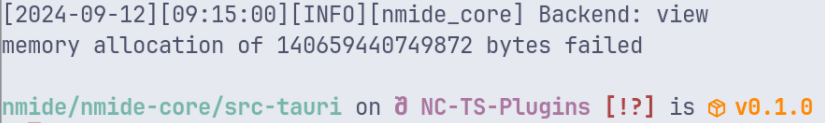
\includegraphics[width=0.8\textwidth]{./pics/memory-allocation-zoomed.png}
    %\caption{Stress Testing}
  \end{figure}
  It's just 140.6594 TeraBytes, which is a meager 15 \% of the total memory of NASA's
  supercomputer
\end{frame}

\begin{frame}
  \frametitle{But Can It Run Doom?}
  \begin{itemize}
    \item JavaScript plugin allows for reusing existing JavaScript libraries
  \end{itemize}
\end{frame}

\begin{frame}
  \frametitle{But Can It Run Doom?}
  \begin{itemize}
    \item JavaScript plugin allows for reusing existing JavaScript libraries
    \item So, you can play Doom
  \end{itemize}
\end{frame}

\begin{frame}
  \begin{center}
    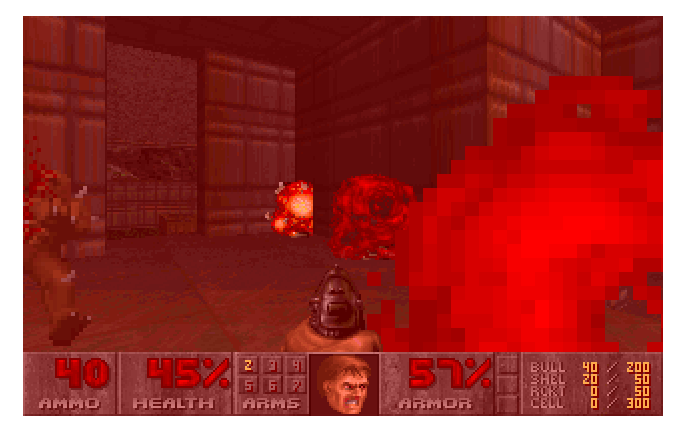
\includegraphics[width=0.95\textwidth]{./pics/doom.png}
    %\caption{Doom using js-dos}
  \end{center}
\end{frame}
